% Generated by Sphinx.
\def\sphinxdocclass{report}
\documentclass[letterpaper,10pt,english]{sphinxmanual}
\usepackage[utf8]{inputenc}
\DeclareUnicodeCharacter{00A0}{\nobreakspace}
\usepackage[T1]{fontenc}
\usepackage{babel}
\usepackage{times}
\usepackage[Bjarne]{fncychap}
\usepackage{longtable}
\usepackage{sphinx}
\usepackage{multirow}


\title{Netzob Documentation}
\date{January 31, 2013}
\release{0.4.1}
\author{Frédéric Guihéry, Georges Bossert}
\newcommand{\sphinxlogo}{}
\renewcommand{\releasename}{Release}
\makeindex

\makeatletter
\def\PYG@reset{\let\PYG@it=\relax \let\PYG@bf=\relax%
    \let\PYG@ul=\relax \let\PYG@tc=\relax%
    \let\PYG@bc=\relax \let\PYG@ff=\relax}
\def\PYG@tok#1{\csname PYG@tok@#1\endcsname}
\def\PYG@toks#1+{\ifx\relax#1\empty\else%
    \PYG@tok{#1}\expandafter\PYG@toks\fi}
\def\PYG@do#1{\PYG@bc{\PYG@tc{\PYG@ul{%
    \PYG@it{\PYG@bf{\PYG@ff{#1}}}}}}}
\def\PYG#1#2{\PYG@reset\PYG@toks#1+\relax+\PYG@do{#2}}

\expandafter\def\csname PYG@tok@gd\endcsname{\def\PYG@tc##1{\textcolor[rgb]{0.63,0.00,0.00}{##1}}}
\expandafter\def\csname PYG@tok@gu\endcsname{\let\PYG@bf=\textbf\def\PYG@tc##1{\textcolor[rgb]{0.50,0.00,0.50}{##1}}}
\expandafter\def\csname PYG@tok@gt\endcsname{\def\PYG@tc##1{\textcolor[rgb]{0.00,0.25,0.82}{##1}}}
\expandafter\def\csname PYG@tok@gs\endcsname{\let\PYG@bf=\textbf}
\expandafter\def\csname PYG@tok@gr\endcsname{\def\PYG@tc##1{\textcolor[rgb]{1.00,0.00,0.00}{##1}}}
\expandafter\def\csname PYG@tok@cm\endcsname{\let\PYG@it=\textit\def\PYG@tc##1{\textcolor[rgb]{0.25,0.50,0.56}{##1}}}
\expandafter\def\csname PYG@tok@vg\endcsname{\def\PYG@tc##1{\textcolor[rgb]{0.73,0.38,0.84}{##1}}}
\expandafter\def\csname PYG@tok@m\endcsname{\def\PYG@tc##1{\textcolor[rgb]{0.13,0.50,0.31}{##1}}}
\expandafter\def\csname PYG@tok@mh\endcsname{\def\PYG@tc##1{\textcolor[rgb]{0.13,0.50,0.31}{##1}}}
\expandafter\def\csname PYG@tok@cs\endcsname{\def\PYG@tc##1{\textcolor[rgb]{0.25,0.50,0.56}{##1}}\def\PYG@bc##1{\setlength{\fboxsep}{0pt}\colorbox[rgb]{1.00,0.94,0.94}{\strut ##1}}}
\expandafter\def\csname PYG@tok@ge\endcsname{\let\PYG@it=\textit}
\expandafter\def\csname PYG@tok@vc\endcsname{\def\PYG@tc##1{\textcolor[rgb]{0.73,0.38,0.84}{##1}}}
\expandafter\def\csname PYG@tok@il\endcsname{\def\PYG@tc##1{\textcolor[rgb]{0.13,0.50,0.31}{##1}}}
\expandafter\def\csname PYG@tok@go\endcsname{\def\PYG@tc##1{\textcolor[rgb]{0.19,0.19,0.19}{##1}}}
\expandafter\def\csname PYG@tok@cp\endcsname{\def\PYG@tc##1{\textcolor[rgb]{0.00,0.44,0.13}{##1}}}
\expandafter\def\csname PYG@tok@gi\endcsname{\def\PYG@tc##1{\textcolor[rgb]{0.00,0.63,0.00}{##1}}}
\expandafter\def\csname PYG@tok@gh\endcsname{\let\PYG@bf=\textbf\def\PYG@tc##1{\textcolor[rgb]{0.00,0.00,0.50}{##1}}}
\expandafter\def\csname PYG@tok@ni\endcsname{\let\PYG@bf=\textbf\def\PYG@tc##1{\textcolor[rgb]{0.84,0.33,0.22}{##1}}}
\expandafter\def\csname PYG@tok@nl\endcsname{\let\PYG@bf=\textbf\def\PYG@tc##1{\textcolor[rgb]{0.00,0.13,0.44}{##1}}}
\expandafter\def\csname PYG@tok@nn\endcsname{\let\PYG@bf=\textbf\def\PYG@tc##1{\textcolor[rgb]{0.05,0.52,0.71}{##1}}}
\expandafter\def\csname PYG@tok@no\endcsname{\def\PYG@tc##1{\textcolor[rgb]{0.38,0.68,0.84}{##1}}}
\expandafter\def\csname PYG@tok@na\endcsname{\def\PYG@tc##1{\textcolor[rgb]{0.25,0.44,0.63}{##1}}}
\expandafter\def\csname PYG@tok@nb\endcsname{\def\PYG@tc##1{\textcolor[rgb]{0.00,0.44,0.13}{##1}}}
\expandafter\def\csname PYG@tok@nc\endcsname{\let\PYG@bf=\textbf\def\PYG@tc##1{\textcolor[rgb]{0.05,0.52,0.71}{##1}}}
\expandafter\def\csname PYG@tok@nd\endcsname{\let\PYG@bf=\textbf\def\PYG@tc##1{\textcolor[rgb]{0.33,0.33,0.33}{##1}}}
\expandafter\def\csname PYG@tok@ne\endcsname{\def\PYG@tc##1{\textcolor[rgb]{0.00,0.44,0.13}{##1}}}
\expandafter\def\csname PYG@tok@nf\endcsname{\def\PYG@tc##1{\textcolor[rgb]{0.02,0.16,0.49}{##1}}}
\expandafter\def\csname PYG@tok@si\endcsname{\let\PYG@it=\textit\def\PYG@tc##1{\textcolor[rgb]{0.44,0.63,0.82}{##1}}}
\expandafter\def\csname PYG@tok@s2\endcsname{\def\PYG@tc##1{\textcolor[rgb]{0.25,0.44,0.63}{##1}}}
\expandafter\def\csname PYG@tok@vi\endcsname{\def\PYG@tc##1{\textcolor[rgb]{0.73,0.38,0.84}{##1}}}
\expandafter\def\csname PYG@tok@nt\endcsname{\let\PYG@bf=\textbf\def\PYG@tc##1{\textcolor[rgb]{0.02,0.16,0.45}{##1}}}
\expandafter\def\csname PYG@tok@nv\endcsname{\def\PYG@tc##1{\textcolor[rgb]{0.73,0.38,0.84}{##1}}}
\expandafter\def\csname PYG@tok@s1\endcsname{\def\PYG@tc##1{\textcolor[rgb]{0.25,0.44,0.63}{##1}}}
\expandafter\def\csname PYG@tok@gp\endcsname{\let\PYG@bf=\textbf\def\PYG@tc##1{\textcolor[rgb]{0.78,0.36,0.04}{##1}}}
\expandafter\def\csname PYG@tok@sh\endcsname{\def\PYG@tc##1{\textcolor[rgb]{0.25,0.44,0.63}{##1}}}
\expandafter\def\csname PYG@tok@ow\endcsname{\let\PYG@bf=\textbf\def\PYG@tc##1{\textcolor[rgb]{0.00,0.44,0.13}{##1}}}
\expandafter\def\csname PYG@tok@sx\endcsname{\def\PYG@tc##1{\textcolor[rgb]{0.78,0.36,0.04}{##1}}}
\expandafter\def\csname PYG@tok@bp\endcsname{\def\PYG@tc##1{\textcolor[rgb]{0.00,0.44,0.13}{##1}}}
\expandafter\def\csname PYG@tok@c1\endcsname{\let\PYG@it=\textit\def\PYG@tc##1{\textcolor[rgb]{0.25,0.50,0.56}{##1}}}
\expandafter\def\csname PYG@tok@kc\endcsname{\let\PYG@bf=\textbf\def\PYG@tc##1{\textcolor[rgb]{0.00,0.44,0.13}{##1}}}
\expandafter\def\csname PYG@tok@c\endcsname{\let\PYG@it=\textit\def\PYG@tc##1{\textcolor[rgb]{0.25,0.50,0.56}{##1}}}
\expandafter\def\csname PYG@tok@mf\endcsname{\def\PYG@tc##1{\textcolor[rgb]{0.13,0.50,0.31}{##1}}}
\expandafter\def\csname PYG@tok@err\endcsname{\def\PYG@bc##1{\setlength{\fboxsep}{0pt}\fcolorbox[rgb]{1.00,0.00,0.00}{1,1,1}{\strut ##1}}}
\expandafter\def\csname PYG@tok@kd\endcsname{\let\PYG@bf=\textbf\def\PYG@tc##1{\textcolor[rgb]{0.00,0.44,0.13}{##1}}}
\expandafter\def\csname PYG@tok@ss\endcsname{\def\PYG@tc##1{\textcolor[rgb]{0.32,0.47,0.09}{##1}}}
\expandafter\def\csname PYG@tok@sr\endcsname{\def\PYG@tc##1{\textcolor[rgb]{0.14,0.33,0.53}{##1}}}
\expandafter\def\csname PYG@tok@mo\endcsname{\def\PYG@tc##1{\textcolor[rgb]{0.13,0.50,0.31}{##1}}}
\expandafter\def\csname PYG@tok@mi\endcsname{\def\PYG@tc##1{\textcolor[rgb]{0.13,0.50,0.31}{##1}}}
\expandafter\def\csname PYG@tok@kn\endcsname{\let\PYG@bf=\textbf\def\PYG@tc##1{\textcolor[rgb]{0.00,0.44,0.13}{##1}}}
\expandafter\def\csname PYG@tok@o\endcsname{\def\PYG@tc##1{\textcolor[rgb]{0.40,0.40,0.40}{##1}}}
\expandafter\def\csname PYG@tok@kr\endcsname{\let\PYG@bf=\textbf\def\PYG@tc##1{\textcolor[rgb]{0.00,0.44,0.13}{##1}}}
\expandafter\def\csname PYG@tok@s\endcsname{\def\PYG@tc##1{\textcolor[rgb]{0.25,0.44,0.63}{##1}}}
\expandafter\def\csname PYG@tok@kp\endcsname{\def\PYG@tc##1{\textcolor[rgb]{0.00,0.44,0.13}{##1}}}
\expandafter\def\csname PYG@tok@w\endcsname{\def\PYG@tc##1{\textcolor[rgb]{0.73,0.73,0.73}{##1}}}
\expandafter\def\csname PYG@tok@kt\endcsname{\def\PYG@tc##1{\textcolor[rgb]{0.56,0.13,0.00}{##1}}}
\expandafter\def\csname PYG@tok@sc\endcsname{\def\PYG@tc##1{\textcolor[rgb]{0.25,0.44,0.63}{##1}}}
\expandafter\def\csname PYG@tok@sb\endcsname{\def\PYG@tc##1{\textcolor[rgb]{0.25,0.44,0.63}{##1}}}
\expandafter\def\csname PYG@tok@k\endcsname{\let\PYG@bf=\textbf\def\PYG@tc##1{\textcolor[rgb]{0.00,0.44,0.13}{##1}}}
\expandafter\def\csname PYG@tok@se\endcsname{\let\PYG@bf=\textbf\def\PYG@tc##1{\textcolor[rgb]{0.25,0.44,0.63}{##1}}}
\expandafter\def\csname PYG@tok@sd\endcsname{\let\PYG@it=\textit\def\PYG@tc##1{\textcolor[rgb]{0.25,0.44,0.63}{##1}}}

\def\PYGZbs{\char`\\}
\def\PYGZus{\char`\_}
\def\PYGZob{\char`\{}
\def\PYGZcb{\char`\}}
\def\PYGZca{\char`\^}
\def\PYGZam{\char`\&}
\def\PYGZlt{\char`\<}
\def\PYGZgt{\char`\>}
\def\PYGZsh{\char`\#}
\def\PYGZpc{\char`\%}
\def\PYGZdl{\char`\$}
\def\PYGZti{\char`\~}
% for compatibility with earlier versions
\def\PYGZat{@}
\def\PYGZlb{[}
\def\PYGZrb{]}
\makeatother

\begin{document}

\maketitle
\tableofcontents
\phantomsection\label{index::doc}


\textbf{Netzob} simplifies the work for security auditors by providing a complete framework for the reverse engineering of communication protocols. It handles different types of protocols : text protocols (like HTTP and IRC), fixed fields protocols (like IP and TCP) and variable fields protocols (like ASN.1 based formats). Netzob is therefore suitable for reversing network protocols, stuctured files and system and process flows (IPC and communication with drivers).

Netzob is provided with modules dedicated to capture data in multiple contexts (network, file, process and kernel data acquisition).


\chapter{The big picture}
\label{index:welcome-to-netzob-s-documentation}\label{index:the-big-picture}
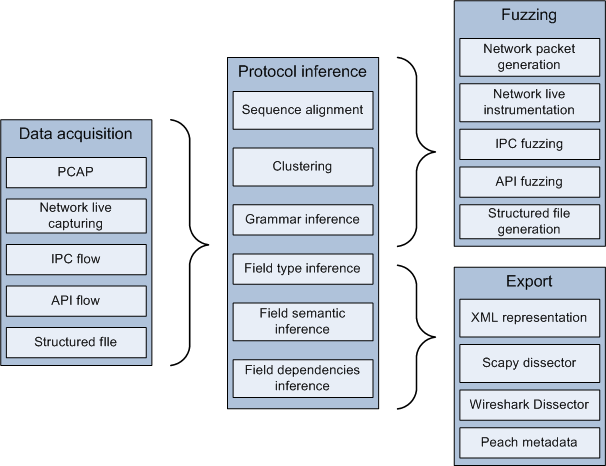
\includegraphics{netzob_archi.png}


\section{Table of contents}
\label{index:table-of-contents}

\subsection{Introduction}
\label{introduction/index:introduction}\label{introduction/index::doc}\label{introduction/index:id1}

\subsection{Import}
\label{import/index:import}\label{import/index::doc}\label{import/index:id1}
Communication protocols can be found is every parts of a system, as shown on the following picture:

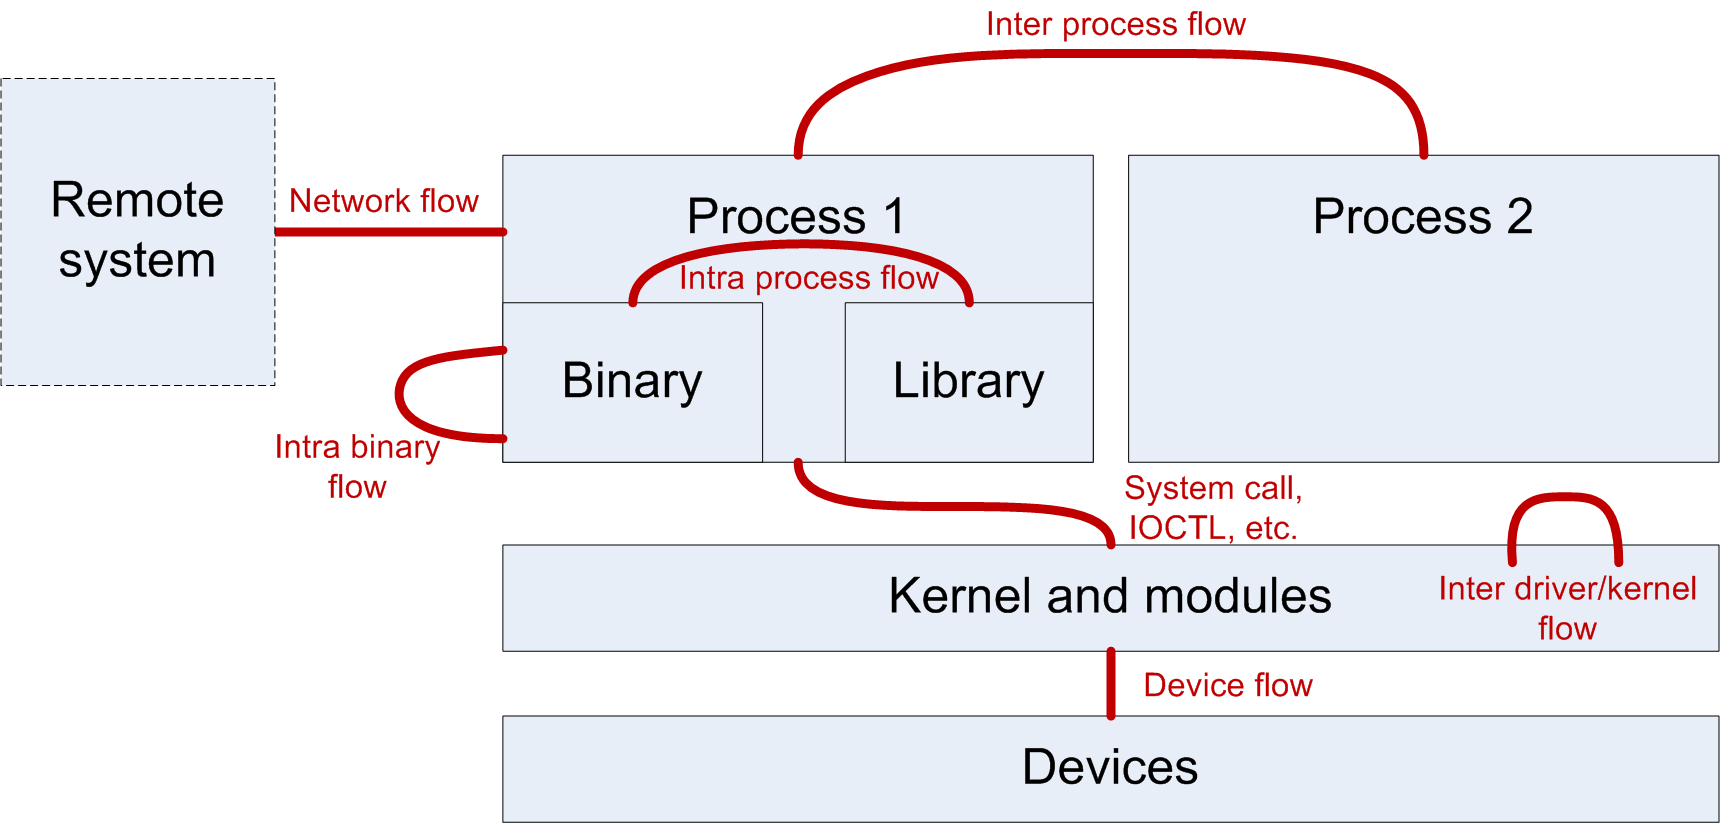
\includegraphics{netzob_comprot.png}

Netzob can handle multiple kinds of input data. Hence, you can analyze network traffic, IPC communications, files structures, etc.

Import can either be done by using a dedicated captor or by providing already captured messages in a specific format.

Current accepted formats are:
\begin{itemize}
\item {} 
PCAP files

\item {} 
Structured files

\item {} 
Netzob XML files (used by Netzob for its internal representation of messages)

\end{itemize}

Current supported captors are:
\begin{itemize}
\item {} 
Network captor, based on the XXX library

\item {} 
Intra Process communication captor (API calls), based on API hooking

\item {} 
Inter Process Communication captor (pipes, shared memory and local sockets), based on system call hooking

\end{itemize}

Imported messages are manipulated by Netzob through specific Python
objects which contains metadata that describes contextual parameters
(timestamp or even IP source/destination for example). All the Python
object that describe messages derived from an abstract object :
AbstractMessage.

The next part of this section details the composition of each message
object.


\subsubsection{AbstractMessage}
\label{import/index:abstractmessage}
All the messages inherits from this definition and therefore has the following parameters :
\begin{itemize}
\item {} 
a unique ID

\item {} 
a data field represented with an array of hex

\end{itemize}


\subsubsection{NetworkMessage}
\label{import/index:networkmessage}
A network message is defined with the following parameters :
\begin{itemize}
\item {} 
a timestamp

\item {} 
the ip source

\item {} 
the ip target

\item {} 
the protocol (TCP/UDP/ICMP...)

\item {} 
the layer 4 source port

\item {} 
the layer 4 target port

\end{itemize}

Definition of a NetworkMessage :


\subsubsection{FileMessage}
\label{import/index:filemessage}
A file message is defined with the following parameters :
\begin{itemize}
\item {} 
a filename

\item {} 
the line number in the file

\item {} 
the creation date of the file

\item {} 
the last modification date of the file

\item {} 
the owner of the file

\item {} 
the size of the file

\end{itemize}

Definition of a NetworkMessage :
\phantomsection\label{import/index:module-netzob.Common.Models.FileMessage}\index{netzob.Common.Models.FileMessage (module)}\index{FileMessage (class in netzob.Common.Models.FileMessage)}

\begin{fulllineitems}
\phantomsection\label{import/index:netzob.Common.Models.FileMessage.FileMessage}\pysiglinewithargsret{\strong{class }\code{netzob.Common.Models.FileMessage.}\bfcode{FileMessage}}{\emph{id}, \emph{timestamp}, \emph{data}, \emph{filename}, \emph{creationDate}, \emph{modificationDate}, \emph{owner}, \emph{size}, \emph{lineNumber}}{}
\end{fulllineitems}


Definition of the factory for XML processing of a FileMessage :
\phantomsection\label{import/index:module-netzob.Common.Models.Factories.FileMessageFactory}\index{netzob.Common.Models.Factories.FileMessageFactory (module)}\index{FileMessageFactory (class in netzob.Common.Models.Factories.FileMessageFactory)}

\begin{fulllineitems}
\phantomsection\label{import/index:netzob.Common.Models.Factories.FileMessageFactory.FileMessageFactory}\pysigline{\strong{class }\code{netzob.Common.Models.Factories.FileMessageFactory.}\bfcode{FileMessageFactory}}
\end{fulllineitems}



\subsection{Modelization}
\label{modelization/index::doc}\label{modelization/index:modelization}\label{modelization/index:id1}

\subsubsection{Definition of a communication protocol}
\label{modelization/index:definition-of-a-communication-protocol}
A communication protocol is as language. A language is defined
through\textasciitilde{}:
\begin{itemize}
\item {} 
its vocabulary (the set of valid words or, in our context, the set
of valid messages) ;

\item {} 
its grammar (the set of valid sentences which, in our context, can
be represented as a protocol state machine, like the TCP state
machine).

\end{itemize}

A word of the vocabular is called a symbol. A symbol represents an
abstract view of a set of similar messages. Similar messages refer to
messages having the same semantic (for example, a TCP SYN message, a
SMTP HELLO message, an ICMP ECHO REQUEST message, etc.).

A symbol is structured following a format, which specifies a sequence
of fields (like the IP format). A field can be splitted into
sub-fields. For example, a payload is a field of a TCP
message. Therefore, by defining a layer as a kind of payload (which is
a specific field), we can retrieve the so-called Ethernet, IP, TCP and
HTTP layers from a raw packet ; each layer having its own vocabular
and grammar.

Field's size can be fixed or variable.
Field's content can be static of dynamic.
Field's content can be basic (a 32 bits integer) or complex (an array).
A field has four attributes\textasciitilde{}:
\begin{itemize}
\item {} 
the type defines its definition domain or set of valid values (16 bits integer, string, etc.) ;

\item {} 
the data description defines the structuration of the field (ASN.1, TSN.1, EBML, etc.) ;

\item {} 
the data encoding defines ... (ASCII, little endian, big endian, XML, EBML, DER, XER, PER, etc.) ;

\item {} 
the semantic defines ... (IP address, port number, URL, email, checksum, etc.).

\end{itemize}

Field's content can be\textasciitilde{}:
\begin{itemize}
\item {} 
static ;

\item {} 
dependant of another field (or a set of fields) of the same message (intra-message dependency) ;

\item {} 
dependant of a field (or a set of fields) of a previous message in the grammar (inter-message dependency) ;

\item {} 
dependant of the environment ;

\item {} 
dependant of the application behaviour (which could depend on the user behaviour) ;

\item {} 
random (the initial value of the TCP sequence number for example).

\end{itemize}


\subsubsection{Modelization in Netzob}
\label{modelization/index:modelization-in-netzob}
Netzob provides a framework for the semi-automated modelization (inference) of communication protocols, i.e. inferring its vocabular and grammar.

{[}INCLURE GRAPH{]}
\begin{itemize}
\item {} \begin{description}
\item[{Vocabular inference}] \leavevmode\begin{itemize}
\item {} 
Message structure inference (based on sequence alignment)

\item {} 
Regoupment of similar message structures

\item {} 
Field type inference

\item {} 
Field dependencies from the same message and from the environment

\item {} 
Field semantic inference

\end{itemize}

\end{description}

\item {} \begin{description}
\item[{Grammar inference}] \leavevmode\begin{itemize}
\item {} 
Identification of the automata of the protocol

\item {} 
Fields dependencies with messages of previous states

\end{itemize}

\end{description}

\end{itemize}

All the functionalities of the framework are detailled in this chapter.


\paragraph{Vocabular inference}
\label{modelization/vocabular::doc}\label{modelization/vocabular:vocabular-inference}\label{modelization/vocabular:vocabular}

\subparagraph{Structure inference}
\label{modelization/vocabular:structure-inference}

\subparagraph{Regoupment of similar structures}
\label{modelization/vocabular:regoupment-of-similar-structures}

\subparagraph{Options during alignment process}
\label{modelization/vocabular:options-during-alignment-process}\begin{itemize}
\item {} 
``read-only” process (do not require a participation in the
communication).

\item {} 
Identify the fixed and dynamic fields of all the messages.

\item {} 
Regroups equivalent messages depending of their fields structures.

\item {} \begin{description}
\item[{Clustering (Regroups equivalent messages using) :}] \leavevmode\begin{itemize}
\item {} 
an UPGMA Algorithm to regroup similar messages

\item {} 
an openMP and MPI implementation

\end{itemize}

\end{description}

\item {} \begin{description}
\item[{Sequencing, Alignment (Identification of fields in messages) :}] \leavevmode\begin{itemize}
\item {} 
Needleman \& Wunsch Implementation

\end{itemize}

\end{description}

\end{itemize}


\subparagraph{Needleman and Wunsch algorithm}
\label{modelization/vocabular:needleman-and-wunsch-algorithm}\begin{itemize}
\item {} 
Originaly a bio-informatic algorithm (sequencing DNA)

\item {} 
Align two messages and identify common patterns and field structure

\item {} 
Computes an alignment score representing the efficiency of the
alignment

\end{itemize}

The following picture shows the sequence alignment of two messages.

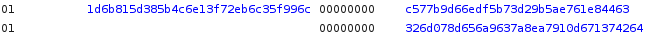
\includegraphics{ExampleOfAligning.png}


\subparagraph{UPGMA algorithm}
\label{modelization/vocabular:upgma-algorithm}\begin{itemize}
\item {} 
Identify equivalent messages based on their alignment score.

\item {} 
Build a hierarchical organization of the messages with the UPGMA
algorithm (Unweighted Pair Group Method with Arithmetic Mean)

\end{itemize}

The following picture shows a regroupment of similar messages based on the result of the clustering process.

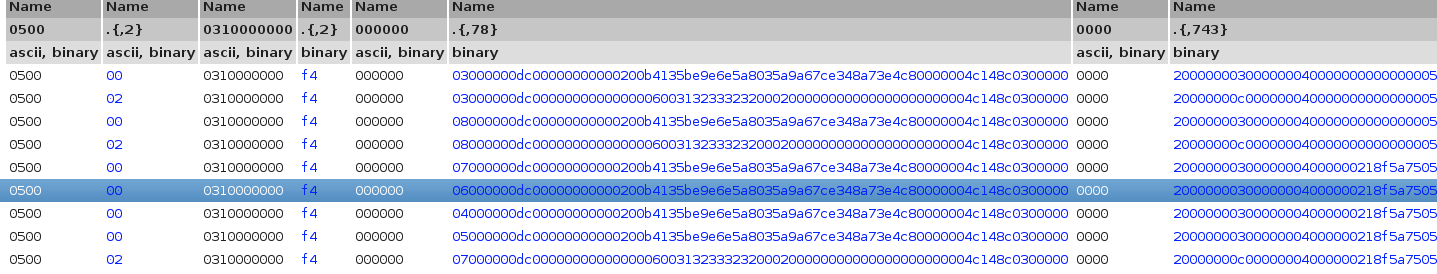
\includegraphics{ExampleOfMultipleAlignment.png}


\subparagraph{Abstraction of a set of message}
\label{modelization/vocabular:abstraction-of-a-set-of-message}
The abstraction is the process of substituting the dynamic fields with their representation as a regex. An example of abstraction is shown on the follinw picture.

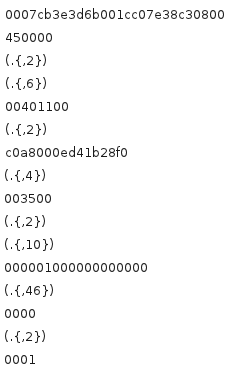
\includegraphics{message_abstraction.png}


\subparagraph{Analyses after alignment process}
\label{modelization/vocabular:analyses-after-alignment-process}
aaa


\subparagraph{Message contextual menu}
\label{modelization/vocabular:message-contextual-menu}
aaa


\subparagraph{Group contextual menu}
\label{modelization/vocabular:group-contextual-menu}
aaa


\subparagraph{Refine regexes}
\label{modelization/vocabular:refine-regexes}
aaa


\subparagraph{Slick regexes}
\label{modelization/vocabular:slick-regexes}
aaa


\subparagraph{Concatenate}
\label{modelization/vocabular:concatenate}
aaa


\subparagraph{Split column}
\label{modelization/vocabular:split-column}
aaa


\subparagraph{Merge columns}
\label{modelization/vocabular:merge-columns}
aaa


\subparagraph{Delete message}
\label{modelization/vocabular:delete-message}
aaa


\subparagraph{Field type inference}
\label{modelization/vocabular:field-type-inference}

\subparagraph{Visualization options}
\label{modelization/vocabular:visualization-options}
aaa


\subparagraph{Type structure contextual menu}
\label{modelization/vocabular:type-structure-contextual-menu}
aaa


\subparagraph{Messages distribution}
\label{modelization/vocabular:messages-distribution}
This function shows a graphical representation of the distribution of bytes per offset for each message of the current group. This function helps to identify entropy variation of each fields. Entropy variation combined with byte distribution help the user to infer the field type.

{[}INCLUDE GRAPH{]}


\subparagraph{Data typing}
\label{modelization/vocabular:data-typing}\begin{itemize}
\item {} \begin{description}
\item[{Primary types}] \leavevmode{[}binary, ascii, num, base64...{]}\begin{itemize}
\item {} 
Definition domain, unique elements and intervals

\item {} 
Data carving (tar gz, png, jpg, ...)

\item {} 
Semantic data identification (emails, IP ...)

\end{itemize}

\end{description}

\end{itemize}


\subparagraph{Domain of definition}
\label{modelization/vocabular:domain-of-definition}
aaa


\subparagraph{Change type representation}
\label{modelization/vocabular:change-type-representation}
aaa


\subparagraph{Field dependencies from the same message and from the environment}
\label{modelization/vocabular:field-dependencies-from-the-same-message-and-from-the-environment}

\subparagraph{Fields dependancies identification}
\label{modelization/vocabular:fields-dependancies-identification}\begin{itemize}
\item {} 
Length fields and associated payloads

\item {} 
Encapsulated messages identifications

\end{itemize}

And from the environment...


\subparagraph{Payload extraction}
\label{modelization/vocabular:payload-extraction}
The function ``Find Size Fields'', as its name suggests, is dedicated to find fields that contain any length value as well as the associated payload. It does this on each group. Netzob supports different encoding of the size field : big and little endian binary values are supported through size of 1, 2 and 4 bytes. The algorithm used to find the size fields and their associated payloads is desribed in the table XXX.

{[}INCLUDE ALGORITHM{]}

The following picture represents the application of the function on a trace example. It shows the automated extraction of the IP and UDP payloads from an Ethernet frame.

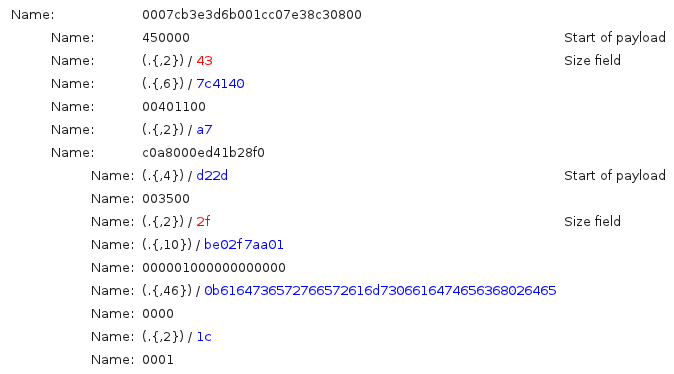
\includegraphics{payload_extraction.png}


\subparagraph{Field semantic inference}
\label{modelization/vocabular:field-semantic-inference}

\subparagraph{Data carving}
\label{modelization/vocabular:data-carving}
Data carving is the process of extracting semantic information from fields or messages. Netzob allows the extraction of the following semantic information :
\begin{itemize}
\item {} 
URL

\item {} 
email

\item {} 
IP address

\end{itemize}

{[}INCLUDE FIGURE{]}


\subparagraph{Search}
\label{modelization/vocabular:search}
aaa


\subparagraph{Properties}
\label{modelization/vocabular:properties}
aaa


\paragraph{Grammar inference}
\label{modelization/grammar:grammar-inference}\label{modelization/grammar:grammar}\label{modelization/grammar::doc}

\subparagraph{Identification of the automata of the protocol}
\label{modelization/grammar:identification-of-the-automata-of-the-protocol}

\subparagraph{Fields dependencies with messages of previous states}
\label{modelization/grammar:fields-dependencies-with-messages-of-previous-states}

\subsection{Vocabular inference}
\label{modelization/vocabular::doc}\label{modelization/vocabular:vocabular-inference}\label{modelization/vocabular:vocabular}

\subsubsection{Structure inference}
\label{modelization/vocabular:structure-inference}

\subsubsection{Regoupment of similar structures}
\label{modelization/vocabular:regoupment-of-similar-structures}

\paragraph{Options during alignment process}
\label{modelization/vocabular:options-during-alignment-process}\begin{itemize}
\item {} 
``read-only” process (do not require a participation in the
communication).

\item {} 
Identify the fixed and dynamic fields of all the messages.

\item {} 
Regroups equivalent messages depending of their fields structures.

\item {} \begin{description}
\item[{Clustering (Regroups equivalent messages using) :}] \leavevmode\begin{itemize}
\item {} 
an UPGMA Algorithm to regroup similar messages

\item {} 
an openMP and MPI implementation

\end{itemize}

\end{description}

\item {} \begin{description}
\item[{Sequencing, Alignment (Identification of fields in messages) :}] \leavevmode\begin{itemize}
\item {} 
Needleman \& Wunsch Implementation

\end{itemize}

\end{description}

\end{itemize}


\paragraph{Needleman and Wunsch algorithm}
\label{modelization/vocabular:needleman-and-wunsch-algorithm}\begin{itemize}
\item {} 
Originaly a bio-informatic algorithm (sequencing DNA)

\item {} 
Align two messages and identify common patterns and field structure

\item {} 
Computes an alignment score representing the efficiency of the
alignment

\end{itemize}

The following picture shows the sequence alignment of two messages.

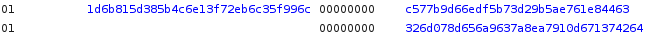
\includegraphics{ExampleOfAligning.png}


\paragraph{UPGMA algorithm}
\label{modelization/vocabular:upgma-algorithm}\begin{itemize}
\item {} 
Identify equivalent messages based on their alignment score.

\item {} 
Build a hierarchical organization of the messages with the UPGMA
algorithm (Unweighted Pair Group Method with Arithmetic Mean)

\end{itemize}

The following picture shows a regroupment of similar messages based on the result of the clustering process.

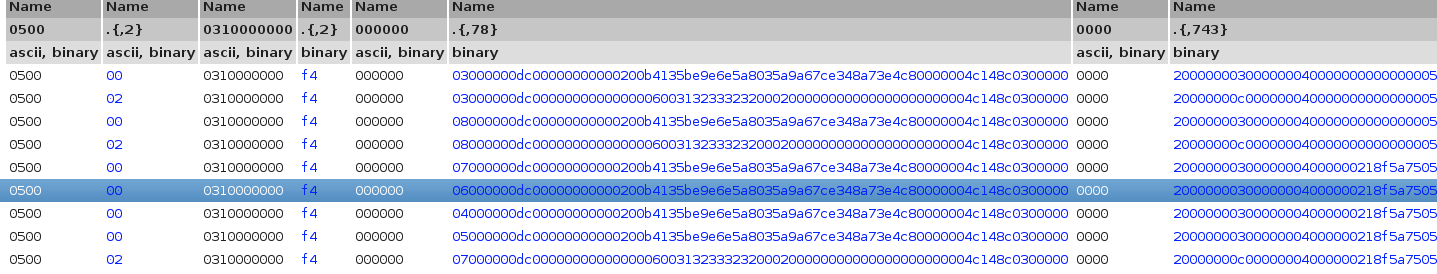
\includegraphics{ExampleOfMultipleAlignment.png}


\paragraph{Abstraction of a set of message}
\label{modelization/vocabular:abstraction-of-a-set-of-message}
The abstraction is the process of substituting the dynamic fields with their representation as a regex. An example of abstraction is shown on the follinw picture.

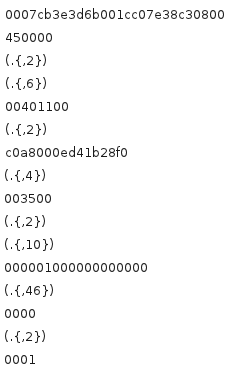
\includegraphics{message_abstraction.png}


\paragraph{Analyses after alignment process}
\label{modelization/vocabular:analyses-after-alignment-process}
aaa


\paragraph{Message contextual menu}
\label{modelization/vocabular:message-contextual-menu}
aaa


\paragraph{Group contextual menu}
\label{modelization/vocabular:group-contextual-menu}
aaa


\paragraph{Refine regexes}
\label{modelization/vocabular:refine-regexes}
aaa


\paragraph{Slick regexes}
\label{modelization/vocabular:slick-regexes}
aaa


\paragraph{Concatenate}
\label{modelization/vocabular:concatenate}
aaa


\paragraph{Split column}
\label{modelization/vocabular:split-column}
aaa


\paragraph{Merge columns}
\label{modelization/vocabular:merge-columns}
aaa


\paragraph{Delete message}
\label{modelization/vocabular:delete-message}
aaa


\subsubsection{Field type inference}
\label{modelization/vocabular:field-type-inference}

\paragraph{Visualization options}
\label{modelization/vocabular:visualization-options}
aaa


\paragraph{Type structure contextual menu}
\label{modelization/vocabular:type-structure-contextual-menu}
aaa


\paragraph{Messages distribution}
\label{modelization/vocabular:messages-distribution}
This function shows a graphical representation of the distribution of bytes per offset for each message of the current group. This function helps to identify entropy variation of each fields. Entropy variation combined with byte distribution help the user to infer the field type.

{[}INCLUDE GRAPH{]}


\paragraph{Data typing}
\label{modelization/vocabular:data-typing}\begin{itemize}
\item {} \begin{description}
\item[{Primary types}] \leavevmode{[}binary, ascii, num, base64...{]}\begin{itemize}
\item {} 
Definition domain, unique elements and intervals

\item {} 
Data carving (tar gz, png, jpg, ...)

\item {} 
Semantic data identification (emails, IP ...)

\end{itemize}

\end{description}

\end{itemize}


\paragraph{Domain of definition}
\label{modelization/vocabular:domain-of-definition}
aaa


\paragraph{Change type representation}
\label{modelization/vocabular:change-type-representation}
aaa


\subsubsection{Field dependencies from the same message and from the environment}
\label{modelization/vocabular:field-dependencies-from-the-same-message-and-from-the-environment}

\paragraph{Fields dependancies identification}
\label{modelization/vocabular:fields-dependancies-identification}\begin{itemize}
\item {} 
Length fields and associated payloads

\item {} 
Encapsulated messages identifications

\end{itemize}

And from the environment...


\paragraph{Payload extraction}
\label{modelization/vocabular:payload-extraction}
The function ``Find Size Fields'', as its name suggests, is dedicated to find fields that contain any length value as well as the associated payload. It does this on each group. Netzob supports different encoding of the size field : big and little endian binary values are supported through size of 1, 2 and 4 bytes. The algorithm used to find the size fields and their associated payloads is desribed in the table XXX.

{[}INCLUDE ALGORITHM{]}

The following picture represents the application of the function on a trace example. It shows the automated extraction of the IP and UDP payloads from an Ethernet frame.

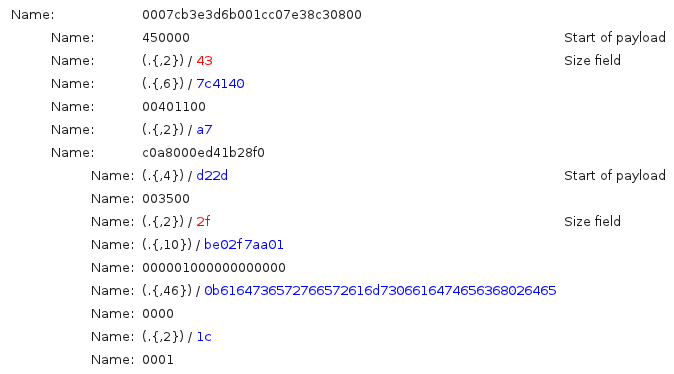
\includegraphics{payload_extraction.png}


\subsubsection{Field semantic inference}
\label{modelization/vocabular:field-semantic-inference}

\paragraph{Data carving}
\label{modelization/vocabular:data-carving}
Data carving is the process of extracting semantic information from fields or messages. Netzob allows the extraction of the following semantic information :
\begin{itemize}
\item {} 
URL

\item {} 
email

\item {} 
IP address

\end{itemize}

{[}INCLUDE FIGURE{]}


\paragraph{Search}
\label{modelization/vocabular:search}
aaa


\paragraph{Properties}
\label{modelization/vocabular:properties}
aaa


\subsection{Grammar inference}
\label{modelization/grammar:grammar-inference}\label{modelization/grammar:grammar}\label{modelization/grammar::doc}

\subsubsection{Identification of the automata of the protocol}
\label{modelization/grammar:identification-of-the-automata-of-the-protocol}

\subsubsection{Fields dependencies with messages of previous states}
\label{modelization/grammar:fields-dependencies-with-messages-of-previous-states}

\subsection{Export}
\label{export/index:export}\label{export/index::doc}\label{export/index:id1}
Netzob supports the export of the modelization of the protocol in the following formats:
* XML meta representation
* Dedicated Scapy Dissector
* Dedicated Wireshark Dissector

Each export format in described in this chapter.


\subsubsection{XML Export}
\label{export/index:xml-export}

\subsubsection{Scapy Dissector}
\label{export/index:scapy-dissector}
The Scapy documentation about building new dissectors is available at the following address:

\href{http://www.secdev.org/projects/scapy/doc/build\_dissect.html}{http://www.secdev.org/projects/scapy/doc/build\_dissect.html}


\subsubsection{Wireshark Dissector}
\label{export/index:wireshark-dissector}
The Wireshark documentation about building new dissectors is available at the following address:

\href{http://www.wireshark.org/docs/wsdg\_html\_chunked/ChDissectAdd.html}{http://www.wireshark.org/docs/wsdg\_html\_chunked/ChDissectAdd.html}


\subsection{Simulation}
\label{simulation/index:id1}\label{simulation/index::doc}\label{simulation/index:simulation}
Todo


\subsection{Fuzzing}
\label{fuzzing/index::doc}\label{fuzzing/index:fuzzing}\label{fuzzing/index:id1}\begin{itemize}
\item {} 
Live instrumentation through a dedicated proxy

\item {} \begin{description}
\item[{Possibilities of variations :}] \leavevmode\begin{itemize}
\item {} 
...

\item {} 
...

\end{itemize}

\end{description}

\end{itemize}


\subsection{Annexes}
\label{Annexes/index::doc}\label{Annexes/index:annexes}\label{Annexes/index:id1}

\subsubsection{GOT Poisoning}
\label{Annexes/index:got-poisoning}
This idea has firstly been described by \emph{Ryan O'Neill} in its article \href{http://vx.netlux.org/lib/vrn00.html}{``Modern Day ELF Runtime infection via GOT poisoning''}.

Netzob has the following needs :
\begin{itemize}
\item {} 
inject between an application and its libraries;

\item {} 
runtime injection,

\item {} 
dump any value of the variables which are transfered from an application to a libs and ``vice et versa'',

\item {} 
modify the value of any variables which are transfered from an application to a libs and ``vice et versa'',

\item {} 
hidden approach,

\end{itemize}

Those needs are generated by the following functionalities :
\begin{itemize}
\item {} 
detection of all the running processes ;

\item {} 
filter for dynamically linked processes ;

\item {} 
display the available libs of a process ;

\item {} 
display all the entry functions of a chosen lib ;

\item {} 
inject a proxy between multiple functions of a lib and the application ;

\item {} 
the injected proxy must be controllable (dump and modify variables).

\end{itemize}

As an example, Netzob must be able to :
\begin{itemize}
\item {} 
fetch all the sent and received message in an HTTPS connection ;

\item {} 
modify for fuzzing experiments in an HTTPS connection.

\end{itemize}


\paragraph{Glossary}
\label{Annexes/index:glossary}
First a bit of vocabulary :

\begin{tabulary}{\linewidth}{|L|L|}
\hline
\textbf{
Term
} & \textbf{
Description
}\\\hline

GOT
 & 
Global Offset Table
\\\hline

PLT
 & 
Procedure linking table
\\\hline
\end{tabulary}



\paragraph{How it works}
\label{Annexes/index:how-it-works}
This approach is composed of two object :
\begin{itemize}
\item {} 
an \emph{injector} which has the responsibility to inject the parasite into a running process;

\item {} 
a \emph{parasite} which aims are to dump and or to modify the values of the variable transfered between a process and its libs.

\end{itemize}

And the scenario of the hijacking algorithm is :
\begin{enumerate}
\item {} 
Locate binary of targeted process by parsing /proc/\textless{}pid\textgreater{}/maps

\item {} 
Parse PLT to get desired GOT address

\item {} 
Attach to the process

\item {} 
Find a place to inject the parasite loader shellcode

\item {} 
Inject new code and save original code we are overwriting

\item {} 
Modify EIP (save old EIP) to point to our code

\item {} 
Resume traced process so that it executes our parasite loader shellcode and load our parasite

\item {} 
Reset register, replace original code and allow process to resume

\item {} 
get base address of our parasite from \%eax

\item {} 
find address of parasite function within shared lib by scanning for its code sequence

\item {} 
Retrieve and save value stored in desired GOT address

\item {} 
Modify the return address of the parasite function with the original function address

\item {} 
Overwrite desired GOT address with new value

\item {} 
Detach from process and enjoy

\end{enumerate}


\paragraph{Step1 : Locate binary of targeted process by parsing /proc/\textless{}pid\textgreater{}/maps}
\label{Annexes/index:step1-locate-binary-of-targeted-process-by-parsing-proc-pid-maps}
\textbf{INPUT :}
\begin{itemize}
\item {} 
PID of the process

\end{itemize}

\textbf{OUTPUT :}
\begin{itemize}
\item {} 
the base address of the application

\item {} 
the full path of the binary

\end{itemize}

\textbf{OPERATIONS :}
\begin{itemize}
\item {} 
Parse the file \emph{/proc/\textless{}pid\textgreater{}/maps}.

\end{itemize}


\paragraph{Step2 : Parse PLT to get desired GOT address}
\label{Annexes/index:step2-parse-plt-to-get-desired-got-address}
\textbf{INPUT :}
\begin{itemize}
\item {} 
the full path of the binary

\item {} 
name of the function to hijack

\end{itemize}

\textbf{OUTPUT :}
\begin{itemize}
\item {} 
the GOT address / offset of the function to hijack

\end{itemize}

\textbf{OPERATIONS :}
\begin{itemize}
\item {} 
Parse the binary (like readelf -r does)

\end{itemize}


\paragraph{Step3 : Attach to the process}
\label{Annexes/index:step3-attach-to-the-process}
\textbf{INPUT :}
\begin{itemize}
\item {} 
PID of the process

\end{itemize}

\textbf{OUTPUT :}

\textbf{OPERATIONS :}
\begin{itemize}
\item {} 
Attach to the process using \emph{PTRACE\_ATTACH}

\end{itemize}


\paragraph{Step4 : Find a place to inject the parasite loader shellcode}
\label{Annexes/index:step4-find-a-place-to-inject-the-parasite-loader-shellcode}
\textbf{INPUT :}
\begin{itemize}
\item {} 
base address of the text segment of the process

\item {} 
parasite loader shellcode

\end{itemize}

\textbf{OUTPUT :}
\begin{itemize}
\item {} 
the {[}start-end{]} offset in the text segment for the injection of shellcode

\end{itemize}

\textbf{OPERATIONS :}
\begin{itemize}
\item {} 
Computes the offset in the segment of the injected

\end{itemize}


\paragraph{Step5 : Inject new code and save original code we are overwriting}
\label{Annexes/index:step5-inject-new-code-and-save-original-code-we-are-overwriting}
\textbf{INPUT :}
\begin{itemize}
\item {} 
start offset of the injection in the text

\item {} 
parasite loader shellcode

\end{itemize}

\textbf{OUTPUT :}
\begin{itemize}
\item {} 
the {[}start-end{]} offset in the text segment for the injection of shellcode

\end{itemize}

\textbf{OPERATIONS :}
\begin{itemize}
\item {} 
backup the original code into memory using \emph{ptrace(PTRACE\_PEEKTEXT} ;

\item {} 
load shellcode into text starting at offset using \emph{ptrace(PTRACE\_POKETEXT} ;

\end{itemize}


\paragraph{Step6 : Modify EIP (save old EIP) to point to our code}
\label{Annexes/index:step6-modify-eip-save-old-eip-to-point-to-our-code}
\textbf{INPUT :}
\begin{itemize}
\item {} 
start offset of the injection in the text

\end{itemize}

\textbf{OUTPUT :}

\textbf{OPERATIONS :}
\begin{itemize}
\item {} 
save the registre using \emph{ptrace(PTRACE\_GETREGS} ;

\item {} 
modify reg.eip using \emph{ptrace(PTRACE\_GETREGS} to the start offset

\end{itemize}


\paragraph{Step7 : Resume traced process so that it executes our parasite loader shellcode and load our parasite}
\label{Annexes/index:step7-resume-traced-process-so-that-it-executes-our-parasite-loader-shellcode-and-load-our-parasite}
\textbf{INPUT :}

\textbf{OUTPUT :}

\textbf{OPERATIONS :}
\begin{itemize}
\item {} 
resume execution using \emph{trace(PTRACE\_CONT}

\end{itemize}


\paragraph{Step8 : Reset register, replace original code and allow process to resume}
\label{Annexes/index:step8-reset-register-replace-original-code-and-allow-process-to-resume}
\textbf{INPUT :}

\textbf{OUTPUT :}

\textbf{OPERATIONS :}
\begin{itemize}
\item {} 
wait for the end of application using * wait(NULL);* ;

\item {} 
retrieves the values of the registers and reset them to default ones

\item {} 
detach from process using \emph{ptrace(PTRACE\_DETACH}

\end{itemize}


\subsubsection{What is a workspace ?}
\label{Annexes/index:what-is-a-workspace}
A workspace contains all the resources files associated with the current analysis which includes :
* the repository of automaton,
* the logging configuration,
* the list of available prototypes of functions which can be hijacked,
* the repository of imported traces,
* the global configuration file.


\subsection{API}
\label{API/index:api}\label{API/index::doc}\label{API/index:id1}
API description
\phantomsection\label{API/index:module-netzob.Common.Workspace}\index{netzob.Common.Workspace (module)}\index{Workspace (class in netzob.Common.Workspace)}

\begin{fulllineitems}
\phantomsection\label{API/index:netzob.Common.Workspace.Workspace}\pysiglinewithargsret{\strong{class }\code{netzob.Common.Workspace.}\bfcode{Workspace}}{\emph{name}, \emph{creationDate}, \emph{path}, \emph{pathOfTraces}, \emph{pathOfLogging}, \emph{pathOfPrototypes}, \emph{lastProjectPath=None}, \emph{importedTraces=\{\}}}{}
Class definition of a Workspace

\end{fulllineitems}

\phantomsection\label{API/index:module-netzob.Common.Project}\index{netzob.Common.Project (module)}\index{Project (class in netzob.Common.Project)}

\begin{fulllineitems}
\phantomsection\label{API/index:netzob.Common.Project.Project}\pysiglinewithargsret{\strong{class }\code{netzob.Common.Project.}\bfcode{Project}}{\emph{id}, \emph{name}, \emph{creationDate}, \emph{path}}{}
Class definition of a Project

\end{fulllineitems}


The API section has a complete list of all the classes, methods,
attributes and functions of the \code{netzob} module, together with short
examples for many items.

A day Netzob will have a proper and efficient documentation. But this day, PYTHON will also have one ! :)


\chapter{Indices and tables}
\label{index:indices-and-tables}\begin{itemize}
\item {} 
\emph{genindex}

\item {} 
\emph{modindex}

\item {} 
\emph{search}

\end{itemize}


\renewcommand{\indexname}{Python Module Index}
\begin{theindex}
\def\bigletter#1{{\Large\sffamily#1}\nopagebreak\vspace{1mm}}
\bigletter{n}
\item {\texttt{netzob.Common.Models.Factories.FileMessageFactory}}, \pageref{import/index:module-netzob.Common.Models.Factories.FileMessageFactory}
\item {\texttt{netzob.Common.Models.FileMessage}}, \pageref{import/index:module-netzob.Common.Models.FileMessage}
\item {\texttt{netzob.Common.Project}}, \pageref{API/index:module-netzob.Common.Project}
\item {\texttt{netzob.Common.Workspace}}, \pageref{API/index:module-netzob.Common.Workspace}
\end{theindex}

\renewcommand{\indexname}{Index}
\printindex
\end{document}
